\chapter{Versat API 2.0}
\label{chapter:API}

The Versat API, developed in a previous thesis~\cite{valter:deepversat}, has the ability to conceal
the calls to the hardware to avoid changing the program when the hardware changes. 

In this chapter, the new functions that are part of the Versat API will be discussed. The goal
is to make development for Versat just like writting normal code and to be easy to port code to it just like
CUDA has done the same to run SIMD code on Nvidia GPUs.

\lstinputlisting[label=listing:versathpp,language=C++,frame=single,breaklines=true,firstline=17,lastline=40,caption=Sample Versat API implementation for the Hardware for Mem functional unit]{./Code/versat.hpp}


On figure \ref{newAPI}, a graphic representation of the new API is presented. It has 4 apparent layers (5 if you count the hardware):

\begin{enumerate}
	\item Complex Mathematical API that is automatically optimized for the Versat Setup you chose. No dev work required
	\item Read/Write using VI and VO for simpler setup of the data. Also includes easier FU functions to setup workloads.
	\item Read/Write configurations for inside Versat Data (Int) or DDR to/from VI/VO (Ext).
	\item Versat API 1.0 where each configuration variable needs to be set up individually
	\item No API. Hardware registers where the values are used inside Versat. 
  \end{enumerate}


\begin{figure}[!htbp]
    \centering
    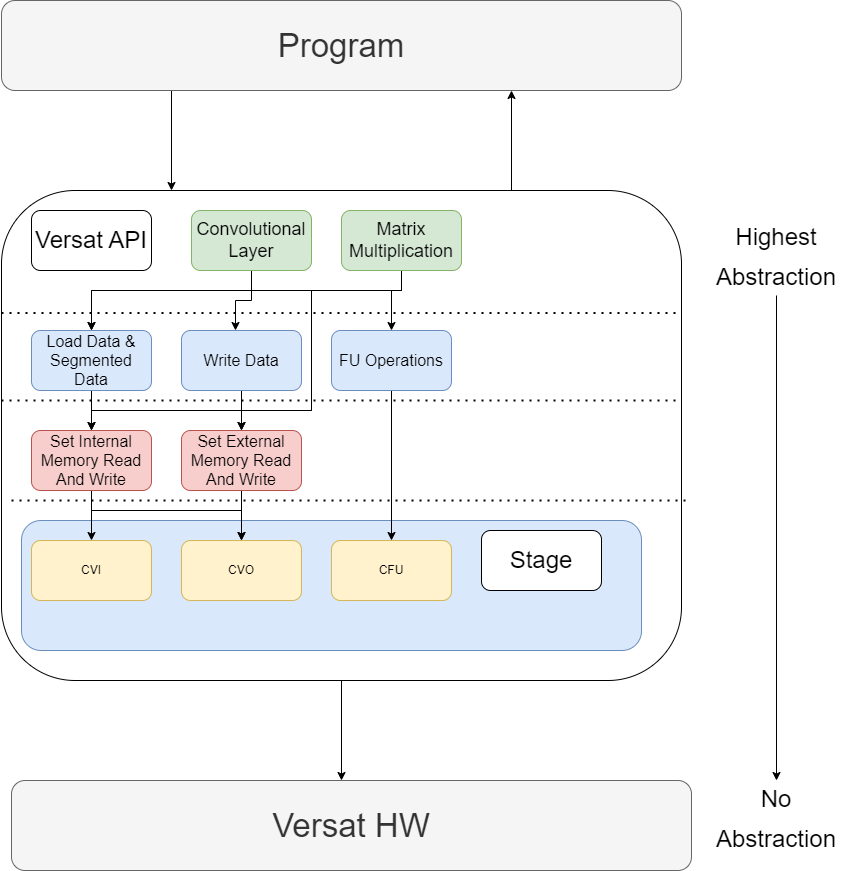
\includegraphics[width=0.7\textwidth]{Figures/VersatMemory.drawio.png}
    \caption{Graphic representation of the new Versat API and it's connections}
    \label{newAPI}
\end{figure} 


\section{Memory Operations API}

When utilizing the VI instead of a MEM, the data transfer happens between the functional unit and a Direct memory access while
on the mem, the CPU writes directly to Versat, wasting CPU cycles. For the API, this means going from a read method that is straightforward
to more configuration methods to set up the read operation from DDR The same happens to Write operations. To address this, 7 functions were created in 2 levels of abstraction:
load\_data(),load\_segmented\_data(),write\_data() that use a lower level functions: set\_IntMem\_Write(),set\_ExtMem\_Write(),set\_IntMem\_Read() and set\_ExtMem\_Read().
The function of the higher abstraction memory functions is to abstract the parameters of the AGU. In the following listing we have one of the implementations
as an example.

Insert Listing of LOAD SEGMENTED DATA

Although this means having to write code with the AGUs in mind
and how they function. To avoid it, a new class was created to also abstract how the AGU counts loops and approximate 
the code to simple C++ code that runs on a CPU.

Insert Listing of ACCUMULATOR


\subsection{}


\section{Software Layers}


Due 18/10

\section{Generic Convolution API}

due 18/10

\subsection{Hardware Configurations}

due 18/10

\subsection{Abstracting Versat Configuration}

due 18/10

\subsection{Convolution Scenarios}

due 18/10




